% !TEX root = main.tex

\section{Testing Architectures}
\label{sec:archs}

We experimented with three types of network architectures, which we call "Inception Net", "Res Net", "Andreas Net". 
For each architecture we will describe their structure, the normalization techniques we applied and the results. 
 
\rhnote{mention that for each network we developed a variant to solve our problem}
\rhnote{how many data points did we use?}
\rhnote{What activation functions did we use}

\rhnote{For normalization we mainly used $L_{1}$ or $L_{2}$ regularization for the fully connected layers and dropout and batch normalization on the convolutional layers.}

\rhnote{Give summary of how these did}

\subsection{Inception Net}

\begin{figure}[t!]
    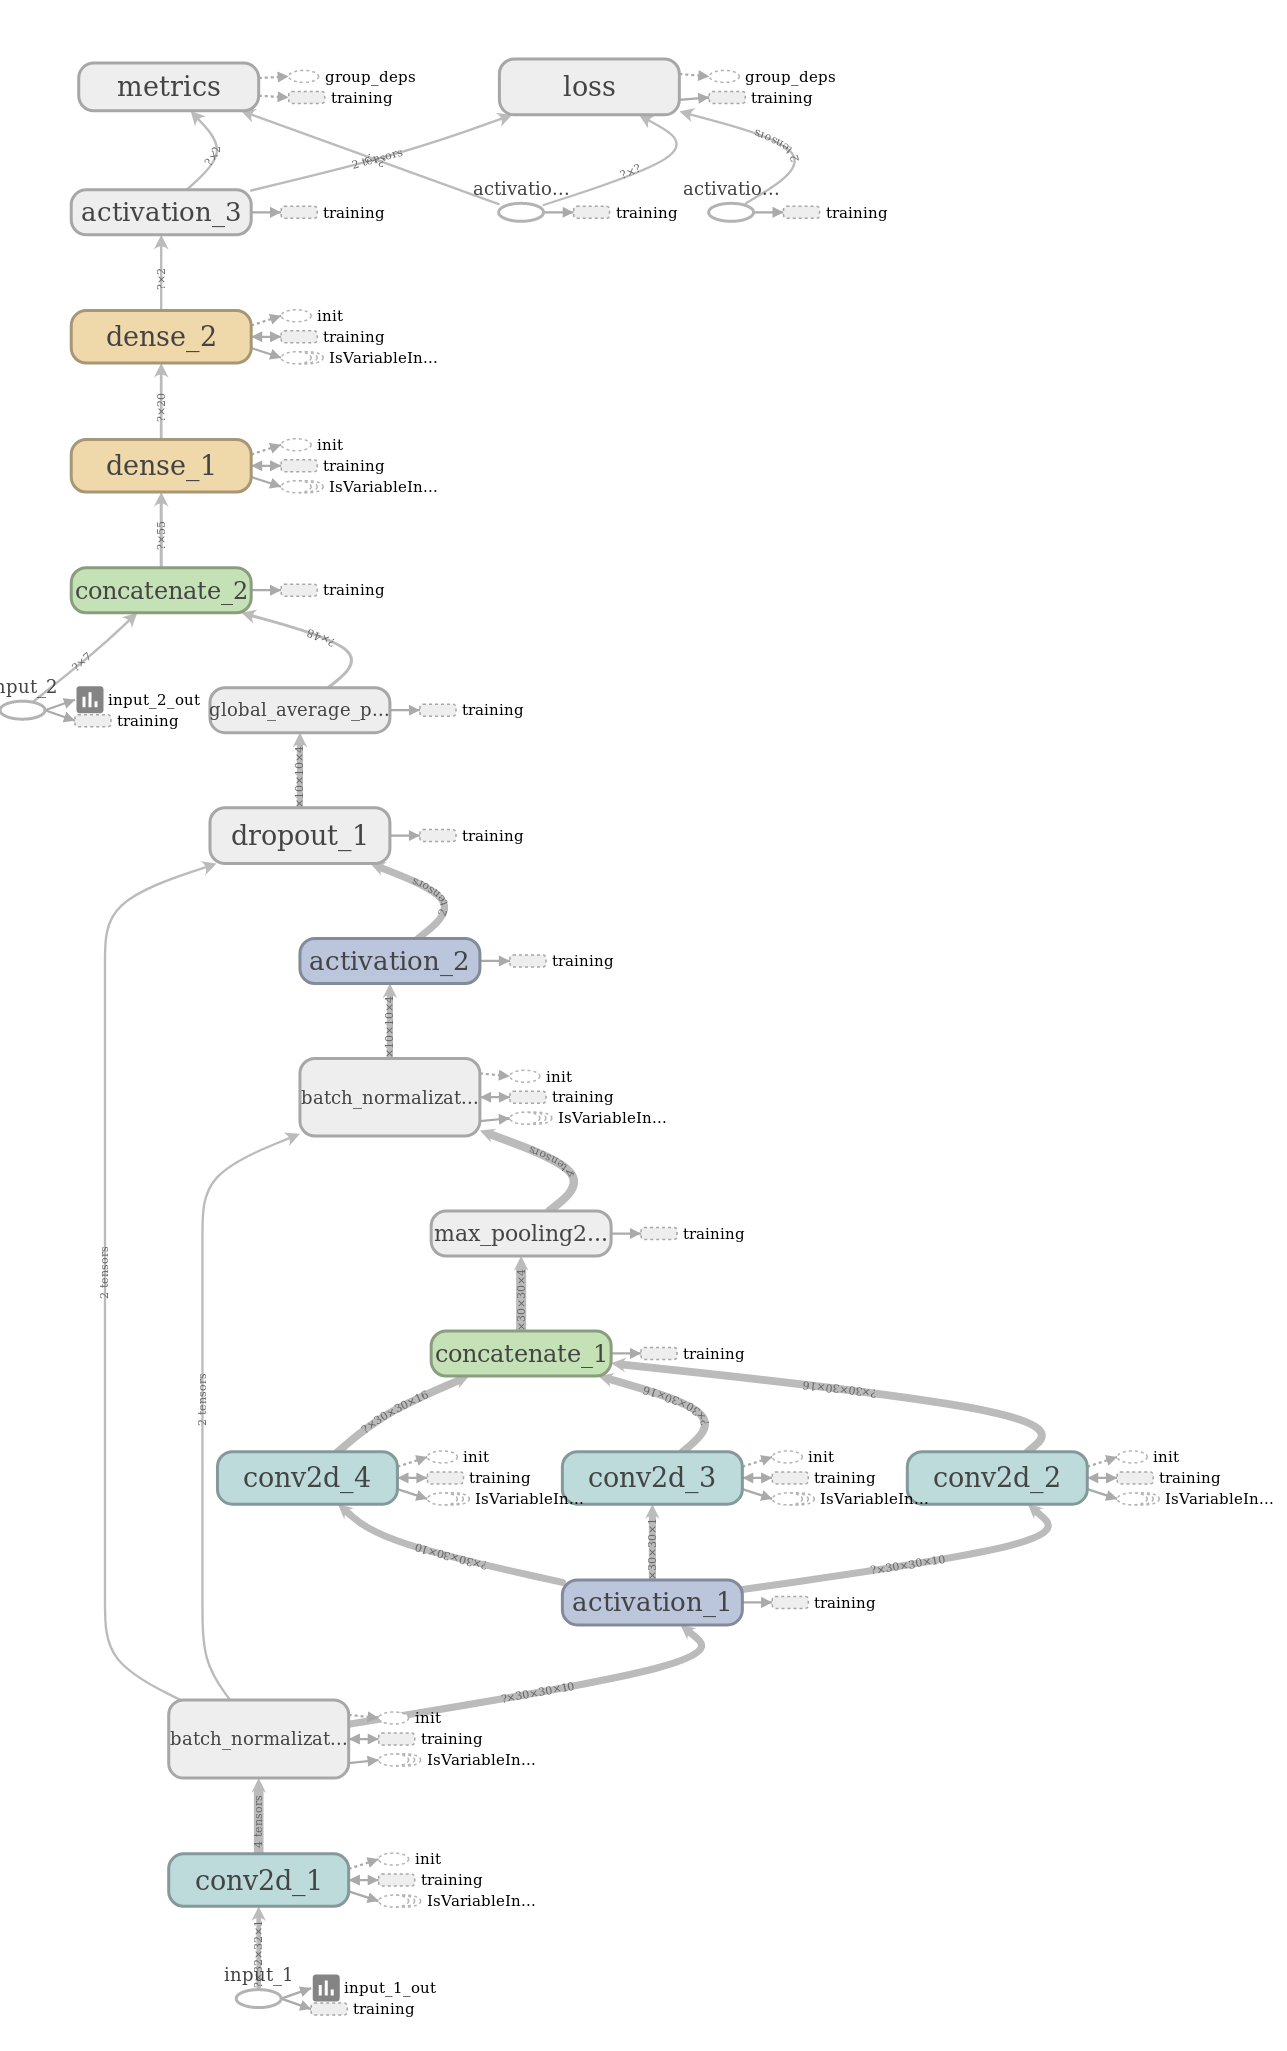
\includegraphics[width=0.99\columnwidth]{figs/inception_net.png}
\caption{Inception Net Architecture} \label{fig:inception_net}
\end{figure}

The first network architecture we will explore is the Inception Network~\cite{szegedy2015going}, visualized in \figref{fig:inception_net}. 
\rhnote{Any intro about this network (ie from the original paper}
This network style was originally designed to increase the depth and width of a network while keeping computational load the same while operating on ImageNet~\cite{deng2009imagenet}. 

The inception network begins with 1 convolution layer in the beginning with 10 filters of size 3x3. 
We apply batch normalization to the output of this layer and pass that to three parallel convolutional layers of sizes 1x1, 3x3, and 5x5, each with 16 filters. 
These outputs are concatenated on the depth dimension and passed through a max pooling layer of 3x3.
We apply batch normalization and a dropout of \rhnote{k\%}. 
The outputs are flattened with global average pooling and then the $z$ value is concatenated before passed to a classifier of one hidden layer of 20 units \rhnote{two FC?}. 

\rhnote{INPUT RESULTS}

\begin{figure*}[t!]
    \centering
    \begin{subfigure}[t]{0.49\textwidth}
        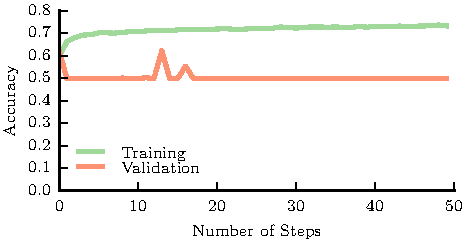
\includegraphics[width=0.9\columnwidth]{figs/inception_accuracy.pdf}
        \caption{Accuracy} \label{fig:accuracy}
        \end{subfigure}
    \begin{subfigure}[t]{0.49\textwidth}
        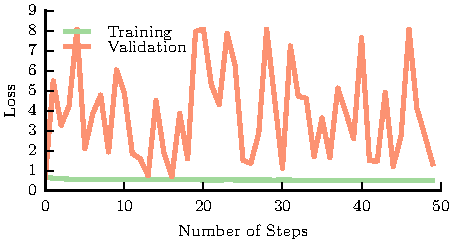
\includegraphics[width=0.9\columnwidth]{figs/inception_loss.pdf}
        \caption{Loss} \label{fig:loss}
    \end{subfigure}
\caption{INSERT CAPTION - inception net} \label{fig:inceptionnet_results}
\end{figure*}


\subsection{Res Net}

\begin{figure}[t!]
    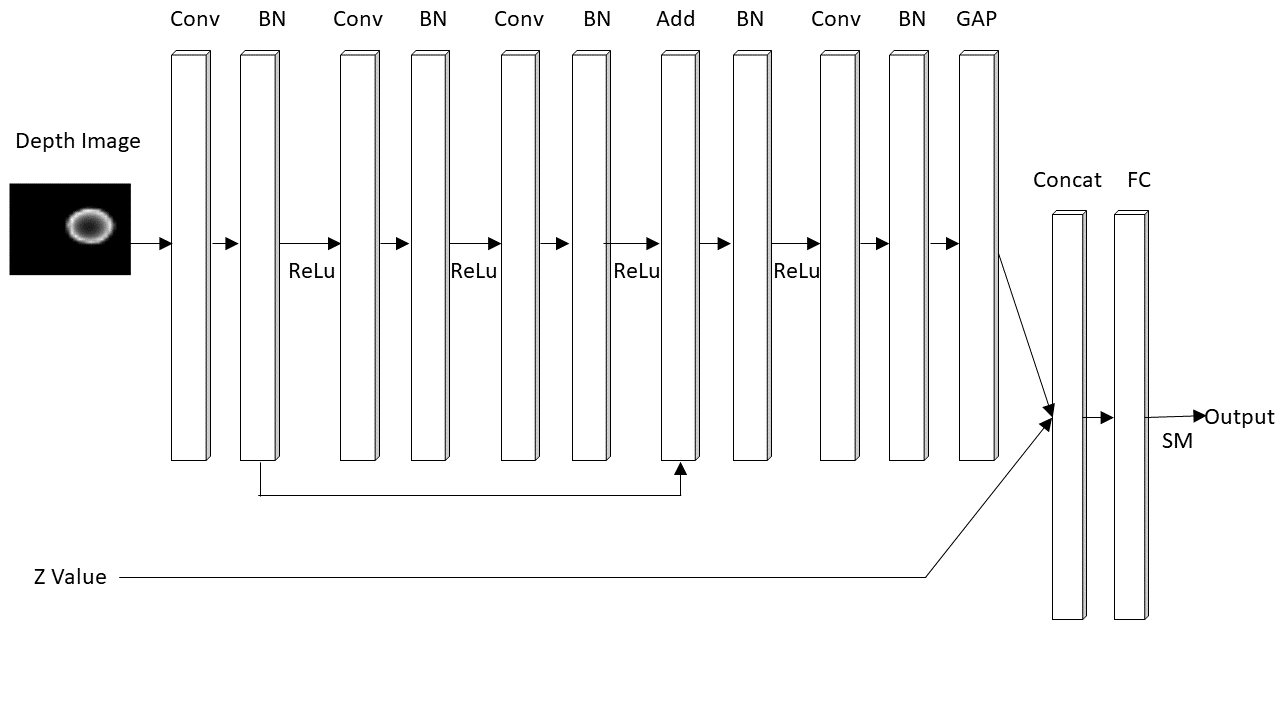
\includegraphics[width=0.99\columnwidth]{figs/res_net.png}
\caption{Res-Net Architecture} \label{fig:res_net}
\end{figure}

Our residual network (called "Res Net" in this discussion) is visualized in \figref{fig:res_net}. 
It consists of one convolutional layer, with 8 filters of size 7x7.
At this point, the output of this layer branches, such that this same output is passed through two more convolution layers of 32 filters 3x3 and 16 filters 1x1 used as dimension reduction. 
The output of these two layers is added to their input and then passed to another convolution layer of 8 filters of 1x1 for further dimension reduction and then flattened with global average pooling. 
After each convolutional layer, we apply batch normalization. 

Like for the other network, the $z$ value is concatenated to this output before passing it to a classifier with a fully connected layer of 10 hidden units.

\rhnote{insert results}

\begin{figure*}[t!]
    \centering
    \begin{subfigure}[t]{0.49\textwidth}
        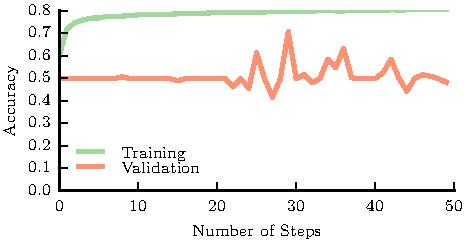
\includegraphics[width=0.9\columnwidth]{figs/res_net_accuracy.pdf}
        \caption{Accuracy} \label{fig:accuracy}
        \end{subfigure}
    \begin{subfigure}[t]{0.49\textwidth}
        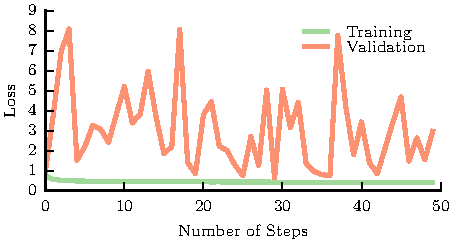
\includegraphics[width=0.9\columnwidth]{figs/res_net_loss.pdf}
        \caption{Loss} \label{fig:loss}
    \end{subfigure}
\caption{INSERT CAPTION - ResNet} \label{fig:resnet_results}
\end{figure*}

\subsection{Andreas Net}

\begin{figure}[t!]
    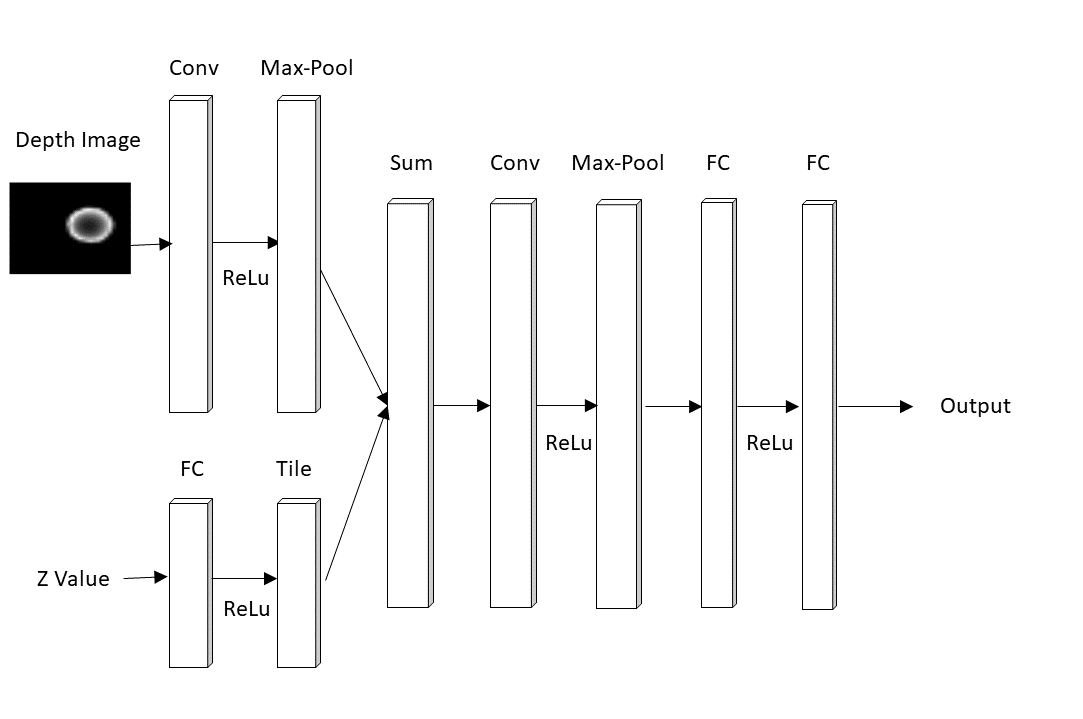
\includegraphics[width=0.99\columnwidth]{figs/andreas_net.png}
\caption{Andreas Net Architecture} \label{fig:andreas_net}
\end{figure}

The last architecture we consider is from~\cite{viereck2017learning} and will be referred to as "Andreas Net". 
It is visualized in \figref{fig:andreas_net}. 
The network, like GQ-CNN, was designed for robotics grasping and uses depth images as input. 
However, \cite{viereck2017learning} creates a closed-loop controller that guides the gripper to the object to be grasped. 
Thus their CNN learns the distance to the nearest grasp function used by the controller. 
Despite its original use as a regression network, we adapt it to our classification task. 

The depth image is passed through one convolutional layer, with 8 filters of size 7x7, and then a max-pooling layer. 
The z-value is passed through a full connected layer and then is tiled.
\rhnote{How does this work for one integer?} \rhnote{explain tiling}
The outputs of each of these are summed before being passed through a convolutional layer with 8 filter of size 7x7 and another max pooling layer. 
Finally, we process through two fully connected layers of size \rhnote{something}. 

\rhnote{results}

\begin{figure*}[t!]
    \centering
    \begin{subfigure}[t]{0.49\textwidth}
        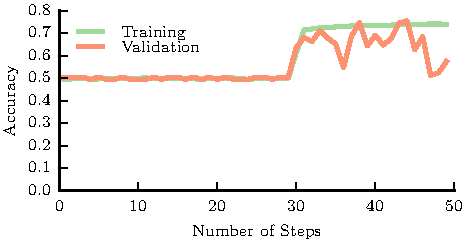
\includegraphics[width=0.9\columnwidth]{figs/andreas_accuracy.pdf}
        \caption{Accuracy} \label{fig:accuracy}
        \end{subfigure}
    \begin{subfigure}[t]{0.49\textwidth}
        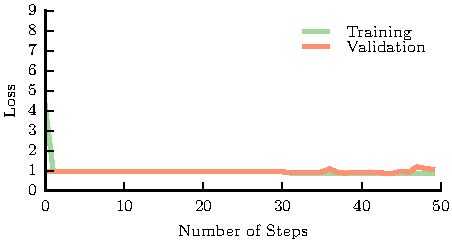
\includegraphics[width=0.9\columnwidth]{figs/andreas_loss.pdf}
        \caption{Loss} \label{fig:loss}
    \end{subfigure}
\caption{INSERT CAPTION - Andreas Net} \label{fig:andreas_results}
\end{figure*}